\documentclass[]{jarticle}          % 一段組
%\documentclass[twocolumn]{jarticle} % 二段組

\textwidth 180mm
\textheight 255mm
\oddsidemargin -12mm
\topmargin -15mm
\columnsep 10mm

%\vspace{0.5cm} % 一段組の場合はコメントアウトした方が体裁がよいx
%] % 一段組の場合はコメントアウトする

\usepackage{styles/labheadings}
\usepackage[dvipdfmx]{graphicx,color}
\usepackage{amsmath,amssymb}
\usepackage{url}
% 追加
\usepackage[hang,small,bf]{caption}
\usepackage[subrefformat=parens]{subcaption}
\usepackage{float}
\captionsetup{compatibility=false}

\input{numerical_definition.tex}
% report.texと同じディレクトリにnumerical_definition.texを入れておけば上の書き方でもいいはずです

\usepackage[
  dvipdfm,
  bookmarks=true,
  bookmarksnumbered=true,
  colorlinks=true]{hyperref}
\AtBeginDvi{\special{pdf:tounicode EUC-UCS2}}

\pagestyle{labheadings}
\headerleft{2次元フロアマップからのシーンの3次元モデルの作成}   % ヘッダの左側のタイトル
\headerright{2024年1月15日}  % ヘッダの右側のタイトル

\begin{document}

%\twocolumn % 一段組の場合はコメントアウトする

\vspace*{2ex}
\begin{center}
 {\Large \bf テクスチャから取得した点特徴の精度評価}\\ % タイトル
 \vspace*{5mm}
 {\large M1 田川幸汰}% 発表者名
\end{center}

%\vspace{0.5cm} % 一段組の場合はコメントアウトした方が体裁がよいx
%] % 一段組の場合はコメントアウトする

%新しく作成したコマンド
% \newcommand{\reffig}[1]{\hyperref[#1]{図\ref{#1}}}
% \newcommand{\refeq}[1]{\hyperref[#1]{式(\ref{#1})}}
% \newcommand{\reftab}[1]{\hyperref[#1]{表\ref{#1}}}
% \newcommand{\refsec}[1]{\hyperref[#1]{\ref{#1}章}}
% \newcommand{\refsubsec}[1]{\hyperref[#1]{\ref{#1}節}}

% 数式
%\begin{equation}
%  数式記述  
%  \label{ラベル名}
%\end{equation}

% 図
% \begin{figure}[!ht]
%   \begin{center}
%     \includegraphics[scale=0.5]{figures/画像ファイル名}
%     \caption{キャプション名}
%     \label{ラベル名}
%   \end{center}
% \end{figure}

% リスト
% \begin{enumerate or itemize}
%   \item 
% \end{enumerate or itemize}
\section{概要}
本資料では、側面テクスチャの歪みを修正し、その結果を反映した3次元モデルの生成結果について示す。
また、生成された3次元モデルに割り当てられたテクスチャから得られた点特徴を用いて実施した自己位置推定の結果を報告する。
さらに、3次元モデルの頂点情報に基づく点特徴とテクスチャ由来の点特徴を比較し、自己位置推定の精度に与える影響を評価した結果を示す。

\section{側面テクスチャの歪みの修正}
本研究では2次元フロアマップを基にシーンの3次元モデルを構築することを目的としており、
その際に側面のテクスチャとしては店舗の正面や壁面が主な対象となると想定している。
店舗の正面や壁面は、一般的に直線的で角度がほとんどない面で構成されており、これらの面を3次元モデル上で自然に再現するためには、
テクスチャの形状についても直線的であることが望ましい。そのため、側面のテクスチャの形状として四角形を採用することが最適であると判断した。

四角形の側面テクスチャを透視投影画像内に描画する際には視野角が広い条件が必要となるため、
先に推定した内部パラメータに視野角の拡大と同等のスケール補正を適用した。これにより、適切な投影が可能となる。
作成した側面テクスチャと、それをもとに生成された3次元モデルを\hyperref[one]{図\ref{one}}に示す。
\begin{figure}[H]
  \begin{center}
    \begin{tabular}{cc}
      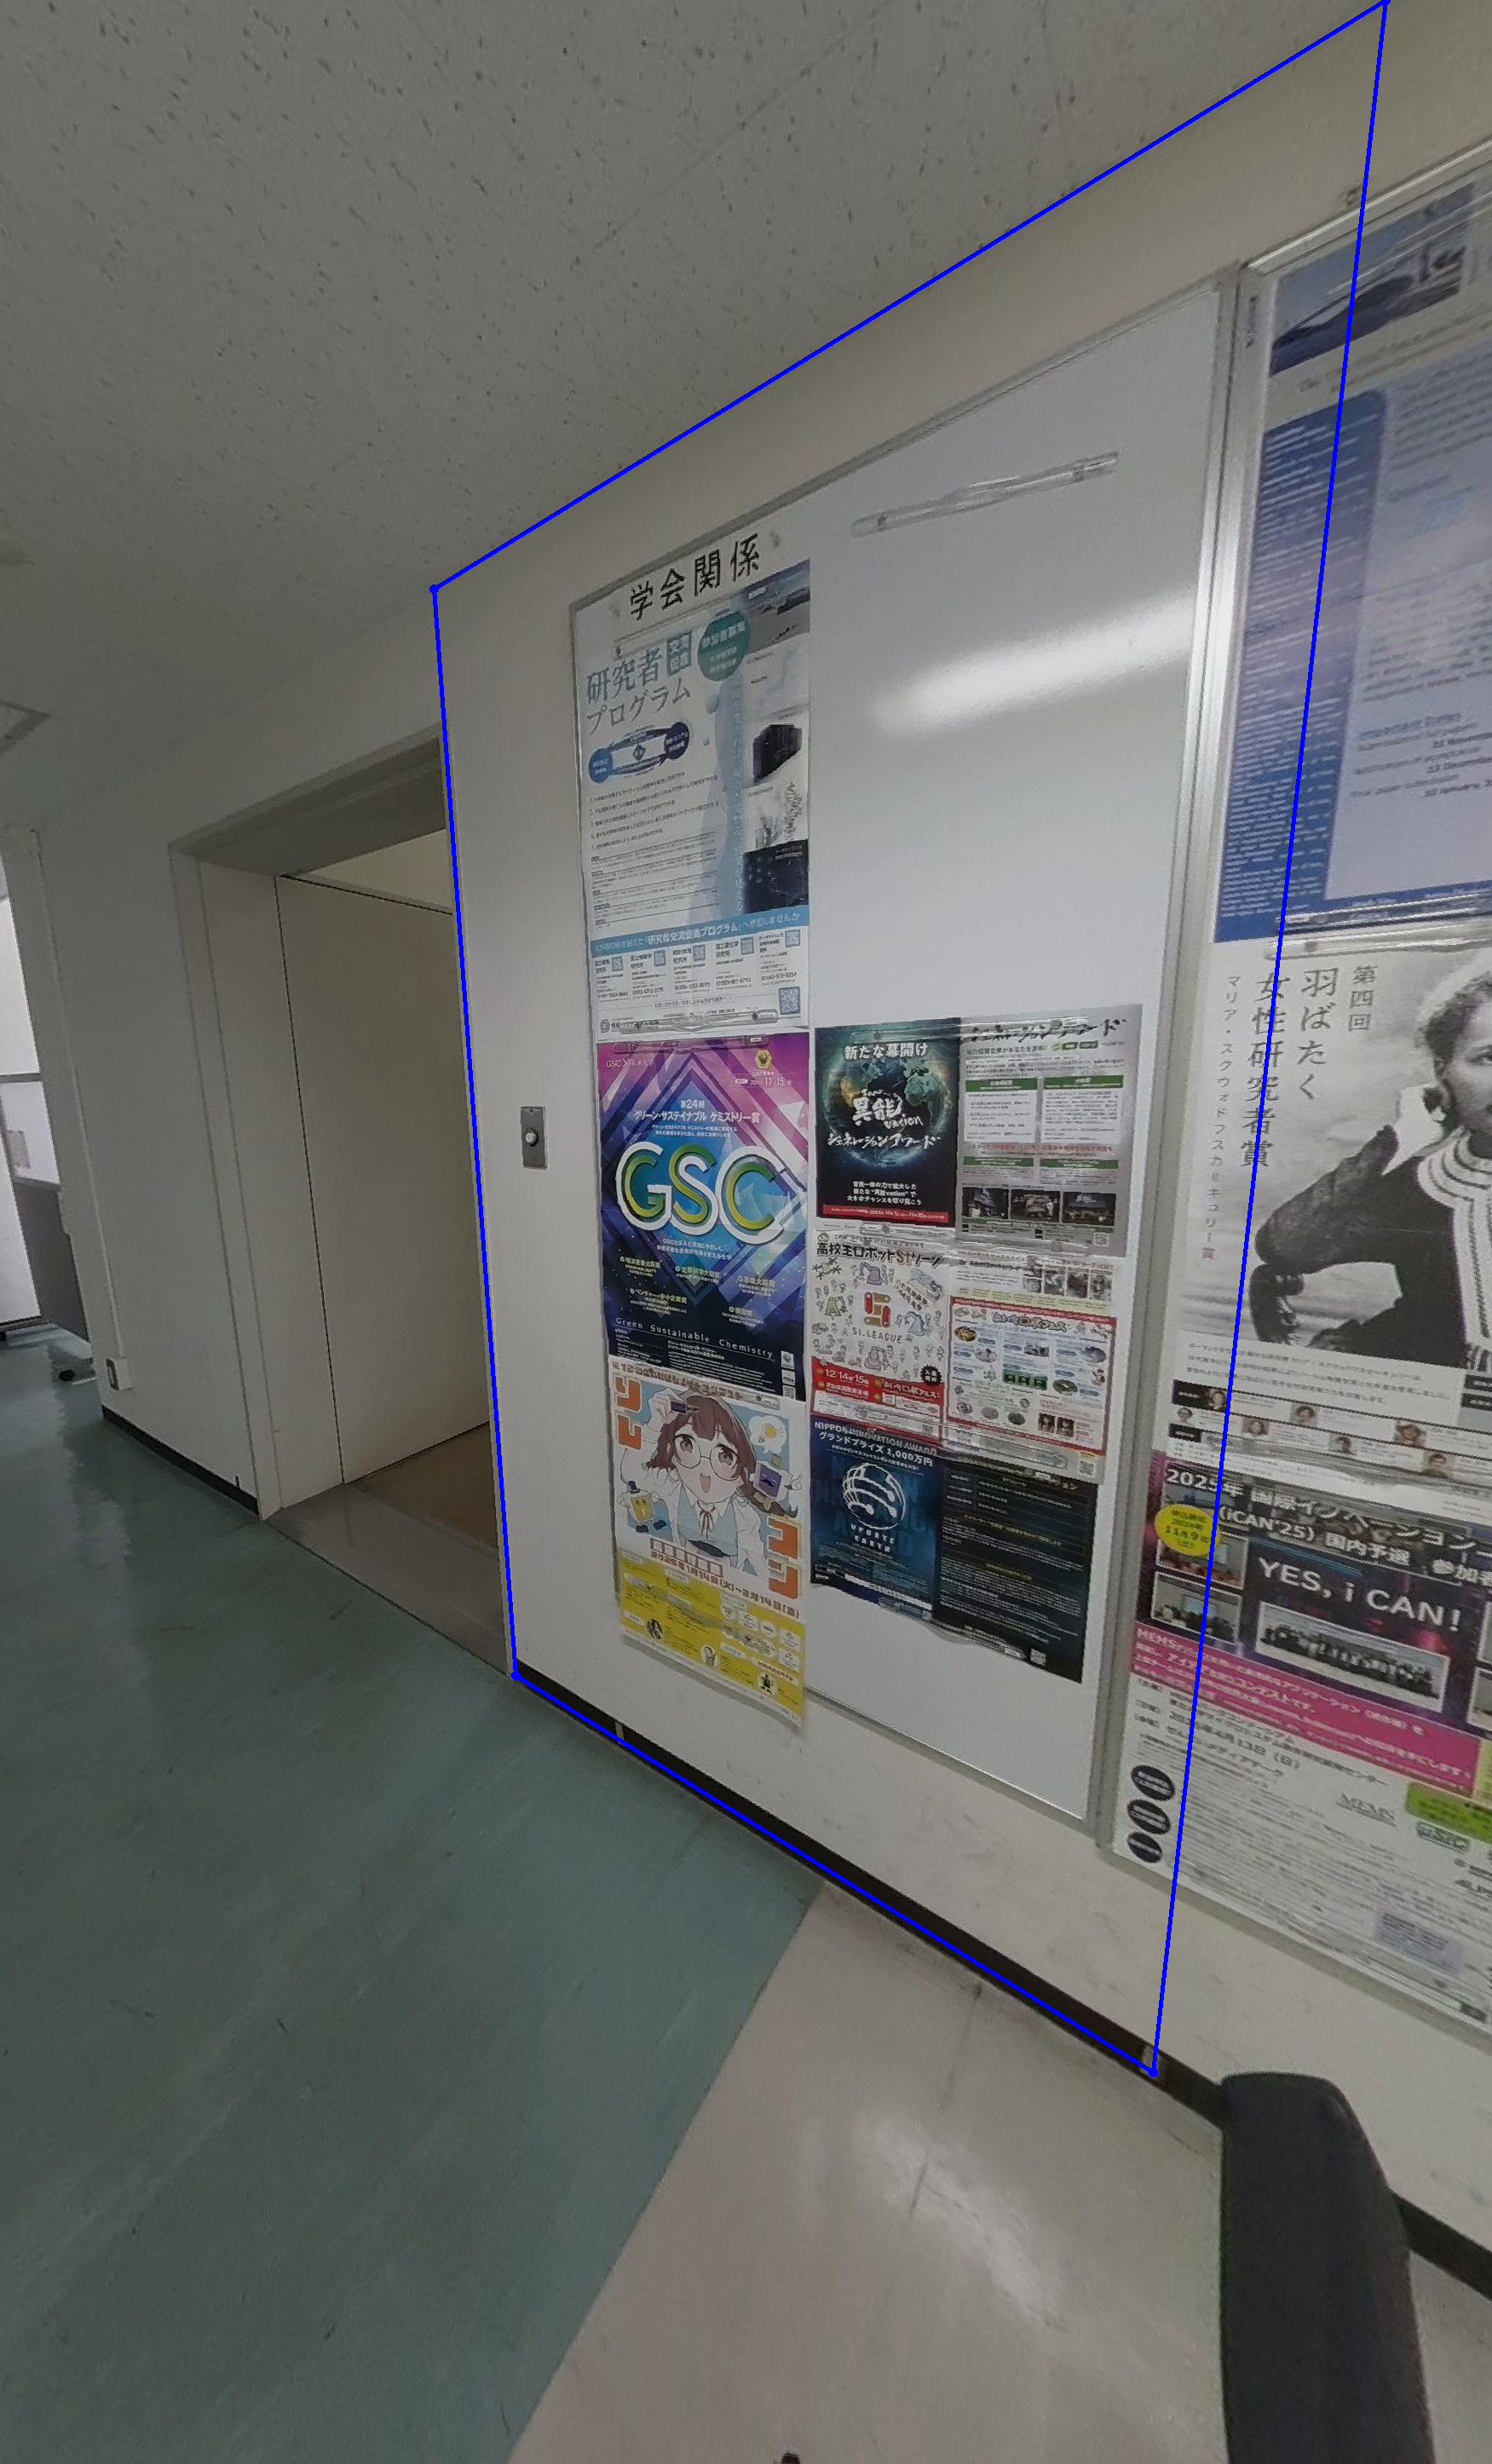
\includegraphics[width=0.4\textwidth]{figures/t.png}&
      \includegraphics[width=0.4\textwidth]{figures/3dmodel_1.png}
    \end{tabular}
  \end{center}
  \caption{側面テクスチャと3次元モデル}
  \label{one}
\end{figure}
図\ref{one}から分かるように、側面テクスチャを得る際に広い視野角を用いた結果、
引き延ばしによって図形の形状変化が発生している。この形状変化により、3次元モデル上で歪みが確認され、モデルの完成度に影響を与えている。
そこで、ホモグラフィー変換によって四角形を長方形となるよう射影変換を行い、テクスチャ画像を割り当てた場合の歪みを補正した。
これらのテクスチャ画像を\hyperref[two]{図\ref{two}}に示す。

\begin{figure}[H]
  \begin{center}
    \begin{tabular}{cc}
      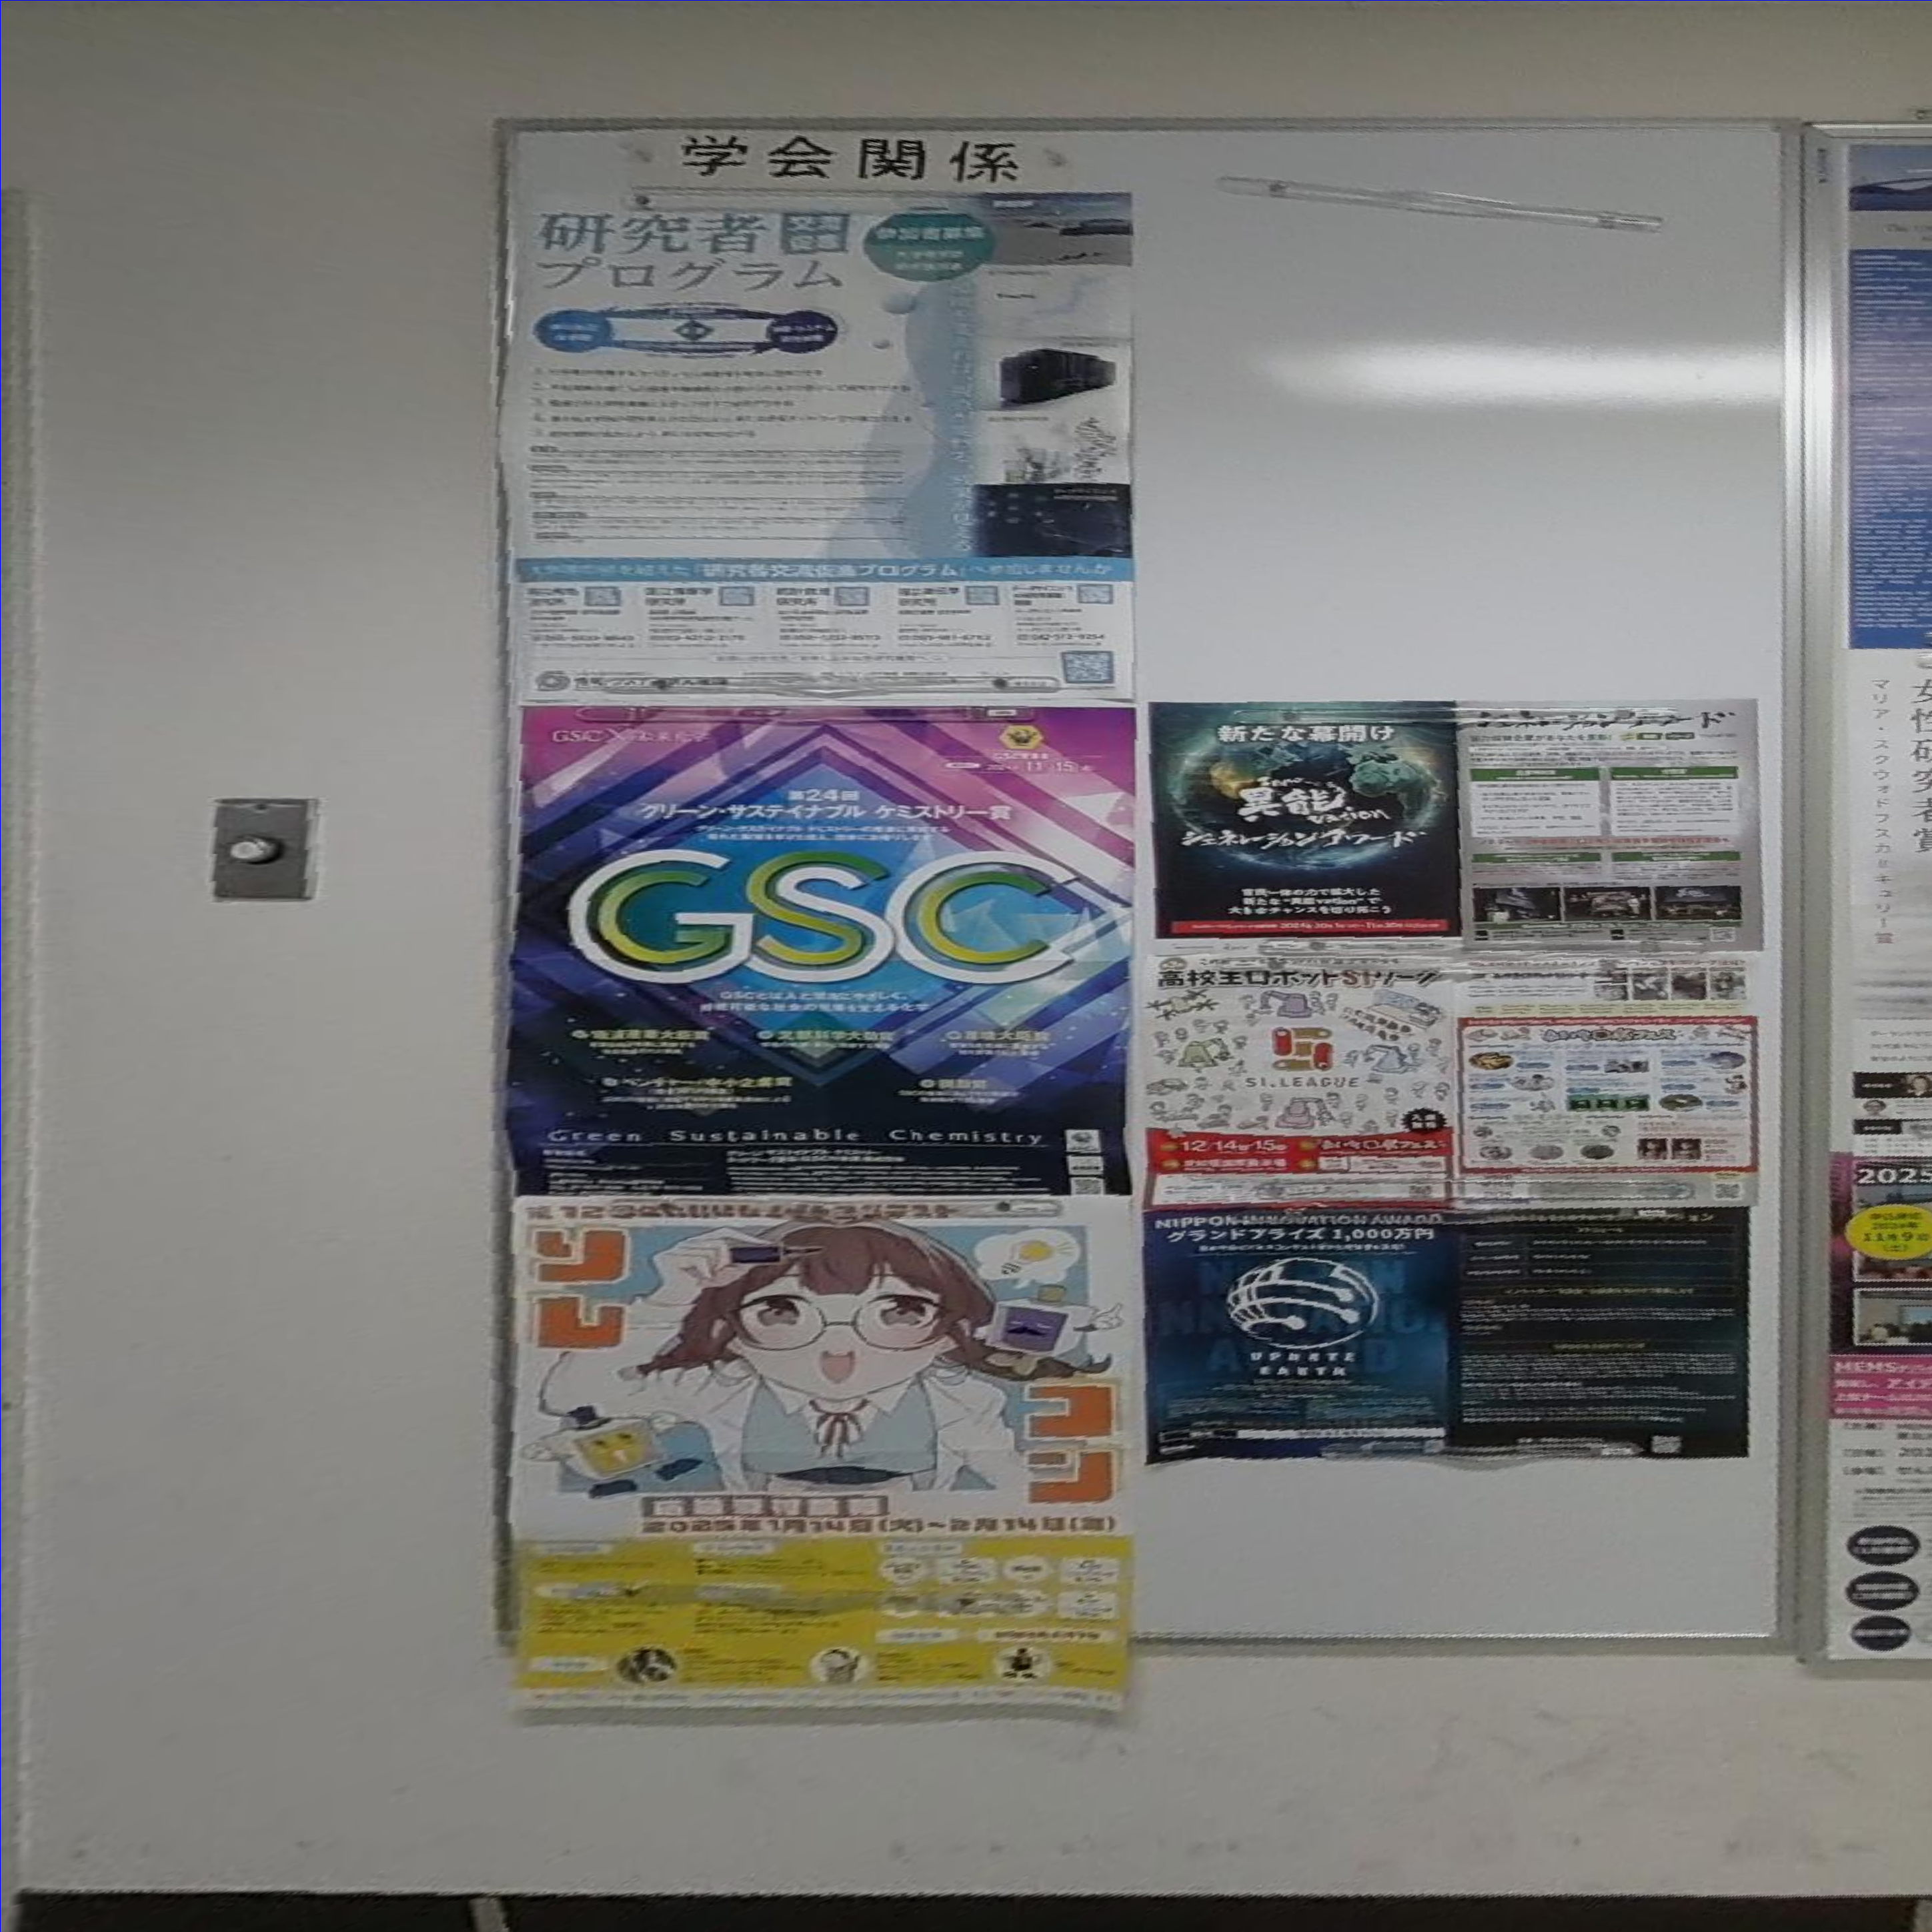
\includegraphics[width=0.4\textwidth]{figures/texture_0_46.png}&
      \includegraphics[width=0.4\textwidth]{figures/texture_2_54.png}\\
    \end{tabular}
  \end{center}
  \caption{テクスチャ画像}
  \label{two}
\end{figure}

これらのテクスチャを用いて生成した3次元モデルを\hyperref[three]{図\ref{three}}に示す。
ホモグラフィー変換の適用により、視野角拡大による歪みを効果的に補正し、
自然な外観を持つ3次元モデルを構築することが可能となった。

\begin{figure}[H]
  \begin{center}
    \begin{tabular}{c}
      \includegraphics[width=0.7\textwidth]{figures/2.png}\\
      \includegraphics[width=0.7\textwidth]{figures/3.png}\\
      \includegraphics[width=0.7\textwidth]{figures/4.png}\\
    \end{tabular}
  \end{center}
  \caption{3次元モデル}
  \label{three}
\end{figure}

\section{テクスチャから得られた点特徴による自己位置推定結果}
テクスチャが正しい位置、角度で3次元モデルに割り当てられているか確認するため、
テクスチャから得られた点特徴と3次元モデルの辺情報に基づく線特徴を用いて自己位置推定を行った。
自己位置推定の大まかな手順を以下に示す。
\begin{enumerate}
  \item 2次元の点特徴と線特徴を入力画像から検出し、対応付けに用いる特徴を手動で選択
  \item 3次元線特徴を3次元モデルの辺情報に基づいて選択
  \item 3次元点特徴を取得する3次元モデルのテクスチャと、対応する2次元座標を選択
  \item テクスチャに投影したスクリーン座標系の2次元座標を世界座標系の3次元座標に変換
  \item 点特徴と線特徴の2次元、3次元対応を基に自己位置を推定
\end{enumerate}
具体的な手法や使用したアルゴリズムについては、後述する各説で説明する。
\subsection{2次元点特徴、線特徴の取得}
入力画像から2次元の点特徴および線特徴を検出する。
対応付けに用いる特徴は、画像から検出された点特徴および線特徴から手動で選択した。
特徴点の検出にはOpenCVのgoodFeaturesToTrackメソッドを使用し、高コントラスト領域を効果的に抽出した。
その結果を\hyperref[four]{図\ref{four}}に示す。
\begin{figure}[H]
  \begin{center}
    \begin{tabular}{c}
      \includegraphics[width=0.5\textwidth]{figures/points1.png}\\
      \includegraphics[width=0.5\textwidth]{figures/lines.png}
    \end{tabular}
  \end{center}
  \caption{2次元点特徴および線特徴}
  \label{four}
\end{figure}
図\ref{four}では、3次元モデルの頂点情報ではなく、面上に存在する特徴点が取得されていることが確認できる。
\subsection{3次元点特徴、線特徴の取得}
3次元線特徴は、3次元モデルの辺情報を基に手動で取得する。
一方、3次元点特徴は、テクスチャに投影されたスクリーン座標系の2次元座標を世界座標系の3次元座標に変換することで得る。この変換過程を以下に示す。
まず、テクスチャから選択した2次元座標を\hyperref[five]{図\ref{five}}に示す。この図では、図\ref{four}(1)に対応した点特徴を選択されている。
\begin{figure}[H]
  \begin{center}
    \begin{tabular}{c}
      \includegraphics[width=0.5\textwidth]{figures/points_texture.png}\\
    \end{tabular}
  \end{center}
  \caption{テクスチャから選択した2次元座標}
  \label{five}
\end{figure}

\subsection{2次元座標から3次元座標への変換}
2次元座標$p$を世界座標系の3次元座標$P$に変換する手順を以下に示す。
\subsubsection{基底ベクトルの計算}
四角形メッシュの頂点の世界座標系の3次元座標を $P_1,P_2,P_3,P_4$ 、
対応するスクリーン座標系の2次元座標を $p_1,p_2,p_3,p_4$ とする。
まず、2次元空間における基底ベクトル $\bU_1,\bU_2$ を式(1)で定義する。
\begin{equation}
  \bU_1 = p_2 - p_1,
  \bU_2 = p_4 - p_1
\end{equation}
また、3次元空間における基底ベクトル $\BU_1,\BU_2$ を式(2)で定義する。
\begin{equation}
  \BU_1 = P_2 - P_1,
  \BU_2 = P_4 - P_1
\end{equation}
\subsubsection{2次元座標の表現}
任意の2次元座標 $p$ を基底ベクトル $\bU_1, \bU_2$ の線型結合として式(3)で表現する。
\begin{equation}
  p = p_1 + \alpha{\bU_1} + \beta{\bU_2}
\end{equation}
この式から係数 $\alpha$、$\beta$ を計算する。
\subsubsection{3次元座標の導出}
世界座標系の3次元座標 $P$ を基底ベクトル $\BU_1, \BU_2$ の線型結合として式(4)で表す。
\begin{equation}
  P= P_1 + \alpha{\BU_1} + \beta{\BU_2}
\end{equation}
ここで、式(3)で求めた $\alpha$、$\beta$ を代入することで、2次元座標 $p$ から世界座標系の3次元座標 $P$ を計算できる。

\subsection{点特徴と線特徴の2次元、3次元対応を基に自己位置を推定}
自己位置推定には、直行射影の共線性および共面性を利用した手法\cite{bib_1}を用いる。
本報告では、テクスチャに基づく点特徴と3次元モデルの頂点情報に基づく点特徴を比較し、それぞれにおける自己位置推定の精度を評価した。
推定結果は\hyperref[table1]{表\ref{table1}}に示す。
また、テクスチャに基づく推定結果をもとに3次元モデル上に結果を表示した様子を\hyperref[six]{図\ref{six}}に示す。
\begin{figure}[H]
  \begin{center}
    \begin{tabular}{lcc}
    & テクスチャ & 3次元モデルの頂点 \\
    誤差x(cm) & 3.09 & 5.13 \\
    誤差y(cm) & -4.29 & -8.90 \\
    誤差z(cm) & -0.91 & 4.14
    \end{tabular}
  \end{center}
  \caption{自己位置推定結果}
  \label{table1}
\end{figure}
\begin{figure}[H]
  \begin{center}
    \begin{tabular}{c}
      \includegraphics[width=0.7\textwidth]{figures/poseestimation.png}\\
    \end{tabular}
  \end{center}
  \caption{自己位置と3次元モデル}
  \label{six}
\end{figure}

推定精度において、テクスチャを使用した場合の方がわずかに優れた結果が得られた。
ただし、これらの誤差は真値ではなく測定値との比較であるため、完全な比較はできない点に留意する必要がある。
テクスチャに基づく特徴点は、コーナー強度が高いため、特徴点としての品質が良好であり、そのため位置推定精度が向上したと考えられる。
一方で、3次元モデルの頂点情報を特徴点に使用する場合、対応する特徴点の検出が難しく、コーナー強度が低いため、特徴点としての品質が低下する傾向が見られた。
これらの結果を踏まえると、テクスチャに基づく点特徴を利用する方法が、自己位置推定においてより有益であると考えられる。

\section{今後の計画}
現在のテクスチャを用いた自己位置推定手法では、特徴点の選択や対応付けが手動で行われているため、実用的な運用には限界がある。
そのため、今後の課題として、入力画像とテクスチャ画像の特徴点を自動で対応付けるアルゴリズムの開発が必要である。
これにより、自己位置推定をより効率的かつ精度高く行えるようにすることを目指す。
具体的には、次のアプローチを検討する。

\begin{enumerate}
  \item \textbf{特徴点の自動対応付けアルゴリズムの開発} \\
  現在は手動で行っている特徴点の選択と対応付けを、自動化するために特徴点検出と特徴量マッチングを統合したアルゴリズムを実装する。
  このために、SIFTやSURFなどの特徴点検出技術を用い、特徴点を自動で対応付けする手法を確立する。
  これにより、位置推定の効率化を図り、リアルタイム処理などで活用できるようにする。

  \item \textbf{フロアマップからの3次元モデル生成} \\
  2次元フロアマップから3次元モデルの頂点と辺のデータを取得し、全方位画像から3次元モデルの面のデータを取得することで、簡便に3次元空間を再現する。

  \item \textbf{生成した3次元モデルを用いた自己位置推定の評価} \\
  生成した3次元モデルを使用した場合に、自己位置推定の精度がどの程度低下するかを実際に測定し、フロアマップから生成されたモデルの実用性を確認する。

  \item \textbf{他の3次元モデル生成手法との比較} \\
  フロアマップから生成した3次元モデルが実用に足る精度を持つ場合、
  次にSfM(Structure from Motion)などの他の3次元モデル生成手法と比較を行う。
  これにより、フロアマップと全方位画像を用いた手法が、どの点で優れているのか、または劣っているのかを定量的に評価する。
  特に、計算時間、精度、構築の容易さなどの観点から比較する。
\end{enumerate}。


\begin{thebibliography}{99}
  \bibitem{bib_1} 菅谷保之,「直交射影の共線性と共面性を用いたカメラ姿勢の推定」
\end{thebibliography}
\end{document}
